\input{../../../Skript_praeambel.tex}

% !TeX spellcheck = en_US

\begin{document}
%Ben�tigte Angaben f�r die Titelseite
\title{Summary of the lecture \\ `Image Processing'\! \\ by Prof. Christian Bauckhage \\ (WiSe 2021/2022)}
%Hier Zeilenumbruch durch \\, da \newline in dieser Umgebung nicht funktioniert.
\author{Fabrice Beaumont \\ Matrikel-Nr: 2747609 \\
Rheinische Friedrich-Wilhelms-Universit�t Bonn}

%Erstellung des Titels
\maketitle
%\tableofcontents
%\listoffigures

%----------------------------------------------------------

%%%%%%%%%%%%%%%%%%%%%%%%%%%%%%%%%%
%%%%% Lecture 01 - 11.10.2021 %%%%
%%%%%%%%%%%%%%%%%%%%%%%%%%%%%%%%%%

% USEFUL LINKS:
% - researchgate.net/project/P3ML-ML-Engineering-Knowledge
% - researchgate.net/project/Machine-Learning-Rhine-Ruhr-ML2R
% - www.b-it-center.de/students/teaching-material/p3ml

% Recommended books:
% - R. Gonzales and R.E. Woods; 'Digital Image Processing'; Prentice Hall, 3rd edition, 2007
% - B. J�hne; 'Digital Image Processing'; Springer, 6th edition, 2005
% - M. Sonka et al.; 'Image Processing, Analysis and Machine Vision'; Cengage, 3rd edition, 2007
% - D.A. Forsyth and J. Ponce; 'Computer Vision: A Modern Approach'; Prentice Hall, 2002
% - R. Hartley and A. Zisserman; 'Multiple View Geometry in Computer Vision'; Cambridge University Press, 2nd edition, 2004
% - G. Wolberg; 'Digital Image Warping'; IEEE Comp. Soc. Press, 1990

\setcounter{chapter}{1}
\chapter{Digital Photography}
%TODO: ANKI bis hier

\section{Image acquisition and digital photography}

(Digital) photography is the practice of visualizing, recording and storing light.

\begin{Definition}[Light]{def:Light}
	\textbf{Light} can be described as both\begin{itemize}
		\item as electromagnetic radiation where energy propagates in form of electromagnetic waves and 
		\item as a particle or quantum phenomenon where photons carry the electromagnetic force.
	\end{itemize}

	Light has a constant \textit{speed} of $c := \SI{299792458}{\sfrac{m}{s}}$. Light can have different \textit{frequency} $\nu$ ($[\SI{}{\per\second}]$) and \textit{wavelength} $\lambda$ ($[\SI{}{\metre}]$), but these properties are reciprocal:
	\begin{equation}
		c = \nu \lambda		\qquad \Big[\frac{\SI{}{\metre}}{\SI{}{\second}}\Big]
	\end{equation}
	
	The \textit{energy} $E$ of light is defined as
	\begin{equation}
		E = h\nu = h\frac{c}{\lambda}		\qquad \Big[\SI{}{\joule}\Big]
	\end{equation}
	where $h = 6.6260689633\times10^{-34} [\SI{}{\joule\second}]$ is the \textbf{Planck's constant}.
\end{Definition}

From these definitions we can derive the relation that light with a high frequency and small wavelength carries more energy.

\begin{figure}[H]
	\centering
	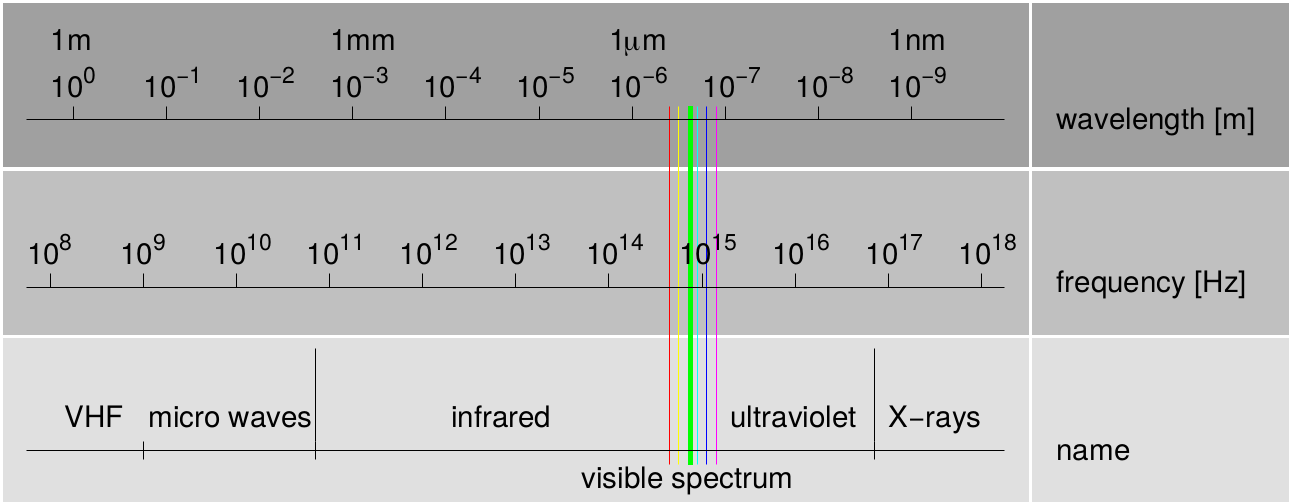
\includegraphics[width=0.8\linewidth]{images/ElectromagneticSpectrumOverview}
	\caption{Overview over the electromagnetic spectrum.}
	\label{fig:electromagneticspectrumoverview}
\end{figure}

There are three ways to visualize light. It can be:\begin{itemize}
	\item \textbf{reflected} (e.g. photographic images or scanned images),
	\item \textbf{absorbed} (e.g. X-ray images) or
	\item \textbf{emitted} (infrared images).
\end{itemize}

There are several ways to record light. Digital (color-)photography relies on CCD cameras. CCD stands for \textbf{charged-coupled device} and describes a semiconductor device consisting of photosensitive elements. Modern consumer cameras have at least $1600\times 1200$ such elements.

Rays of light incident on the camera lens hit the CCD matrix. These photons generate a charge on the CCD elements by freeing electrons. The more light there is, the more electrons are freed. Depending on the camera quality, a single CCD element stores \num[group-separator={,}]{100000} to \num[group-separator={,}]{350000} electrons before saturating. An electric field gathers electrons into packets which are read and quantized into intensity levels. Thus every CCD element records a value of light intensity.

Since the amount of represented intensity levels relates to the needed memory bits per CCD, and since the perception of the human visual system is limited in this regard, typical images typically only store $2^8 = 256$ intensity levels (one byte) per color channel (intensity quantization).

\begin{Definition}[Intensity image]{def:IntensityImage}
	\textbf{Intensity images} (\textbf{grayscale images}) do not contain color information and only display recorded light intensity (luminescence) per pixel in terms of shades of gray.
\end{Definition}

\begin{Definition}[Color image]{def:Color images}
	\textbf{Color images} do contain color information and split the recorded light into basic colors (commonly red, green and blue) from which the appropriate colors can be reconstructed on a display device later. To split the light one can use either a \textbf{trichroic prism} and record each basic color in a separate CCD array, or superimpose a mosaic of color filters (\textbf{Bayer filter}) over a single CCD array. Since the latter technique uses three times less CCD elements it is much cheaper (but also less accurate).
\end{Definition}

\begin{figure}[H]
	\centering
	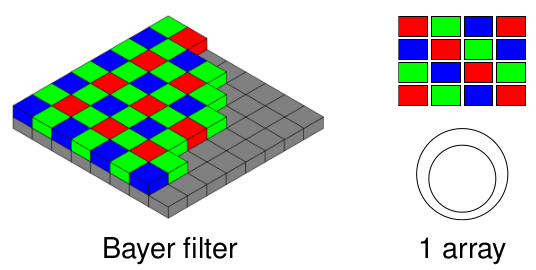
\includegraphics[width=0.45\linewidth]{images/BayerFilter}
	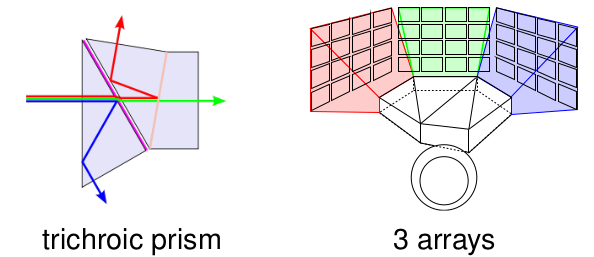
\includegraphics[width=0.45\linewidth]{images/TrichroicPrism}
	\caption{Two techniques of CCD cameras to split recoreded light into three basic colors.}
	\label{fig:ColorImagesCCDTechniques}
\end{figure}

There are several problems with the CCD technology:\begin{itemize}
	\item \textbf{Geometric distortions}. CCD elements are typically not perfectly square. This may necessitate computational correction to compensate for geometric distortions.
	\item \textbf{Blooming}. Overexposure may free to many electrons, which may overflow to neighboring elements and cause highlight effects.
	\item \textbf{Dark noise}. CCD sensors are sensitive to parts of the invisible electromagnetic spectrum (UV or IR radiation) and may thus record invisible apparitions.
\end{itemize}

There are numerous file formats for storing digital images. But these can be separated into two main types of image file formats:\begin{itemize}
	\item vector graphics formats (e.g. SVG, FIG) and
	\item pixmaps (bitmap, raster graphics; e.g. JPG, GIF, PNG, TIFF).
\end{itemize}

\begin{Definition}[PPM format]{def:PPMFormat}
	The \textbf{PPM} (\textbf{portable pixmap}) \textbf{format} stores image data in the following way:\\
	The first four lines in the file format contain:\begin{enumerate}
		\item a magic number (indicating ASCII [P1, P2, P3] or binary [P4, P5, P6] format),
		\item comments,
		\item image width and image height and
		\item the maximum color value (which is the same for all color channels).
	\end{enumerate}
	After these lines, the image data is stored in red-green-blue-triples of hexadecimal values.
\end{Definition}

\begin{figure}[H]
	\centering
	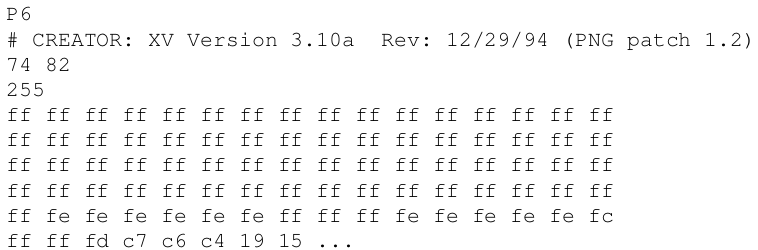
\includegraphics[width=0.8\linewidth]{images/PPMExample}
	\caption{Example header of a PPM file.}
	\label{fig:ppmexample}
\end{figure}

Keep in mind, that there are many different ways of image compression. In general these annihilate information and thus reduce memory requirements.

\section{Representations of digital images}

As explained, a digital image represents digitized and quantized information. The basic element of digital images are called \textbf{pixels} (picture elements), which are (commonly) arranged on a rectangular grid called a \textbf{pixmap}. The \textbf{resolution} of a digital image is expressed in terms of width times height of its pixmap.

Digital images often have an aspect ratio of 4:3 (e.g. $1024\times 768$) or 16:9 (e.g. $1920\times 1080$).

In memory, intensity images are stored in a single pixmap. Color images are stored in three to four pixmaps. One per color channel and a possible $\alpha$-layer. Accordingly, these images can be stored in two-, three- or four-dimensional arrays. Rows and columns of a pixel array are counted from zero and the pixel $p_{0,0}$ is located in the \textit{upper left corner} of the pixel array.

\begin{Definition}[4-Neighborhood]{def:4Neighborhood}
	The \textbf{4-neighborhood} of a pixel is the set of the two vertically and the two horizontally adjacent pixels.
\end{Definition}

\begin{Definition}[8-Neighborhood]{def:8Neighborhood}
	The \textbf{8-neighborhood} of a pixel is the set of the 4-neighborhood and the four diagonally adjacent pixels.
\end{Definition}

\begin{figure}[H]
	\centering
	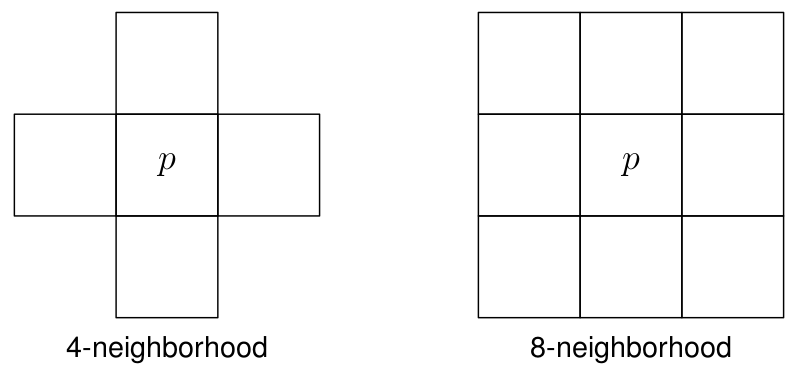
\includegraphics[width=0.7\linewidth]{images/FourAndEightNeighborhood}
	\caption{}
	\label{fig:fourandeightneighborhood}
\end{figure}

Note that the Euclidean distance yields different distances between the pixels in the 8-neighborhood. It is possible to use another metric or another arrangement of the pixelmap (e.g. a hexagonal-grid), but the technically simplest approach with respect to computer memory is the default rectangular grid.

\subsection{Images as functions}

In a digital intensity image, array coordinates $[i,j] \in \{0,\dots,M-1\}\times\{0,\dots,N-1\}$ are mapped to intensity values $p_{i,j}\in \{0,\dots,L-1\}$. Thus one may think of such an image as a \textbf{bi-variate discrete function with finite domain} $f:\IR_+^2\to \IR_+$.

Since the pixels are enumerated from the upper left corner, mapping the planar points $[x_j,y_i]$ to the images array coordinates $[i,j]$ is done as 
\begin{equation}
	[x_i,y_j] \leftrightarrow [j,M-1-i]
\end{equation}

Also, we assume that the two-dimensional point at which an image function is defined are equally spaced. More precise, the horizontal and vertical distances between neighboring point amounts to one:
\begin{equation}
\begin{aligned}
	\delta_x = |x_{j\pm 1}-x_j| = |x \pm 1 - x| = 1\\
	\delta_y = |y_{i\pm 1}-y_j| = |y \pm 1 - y| = 1
\end{aligned}	
\end{equation}

\begin{figure}[H]
	\centering
	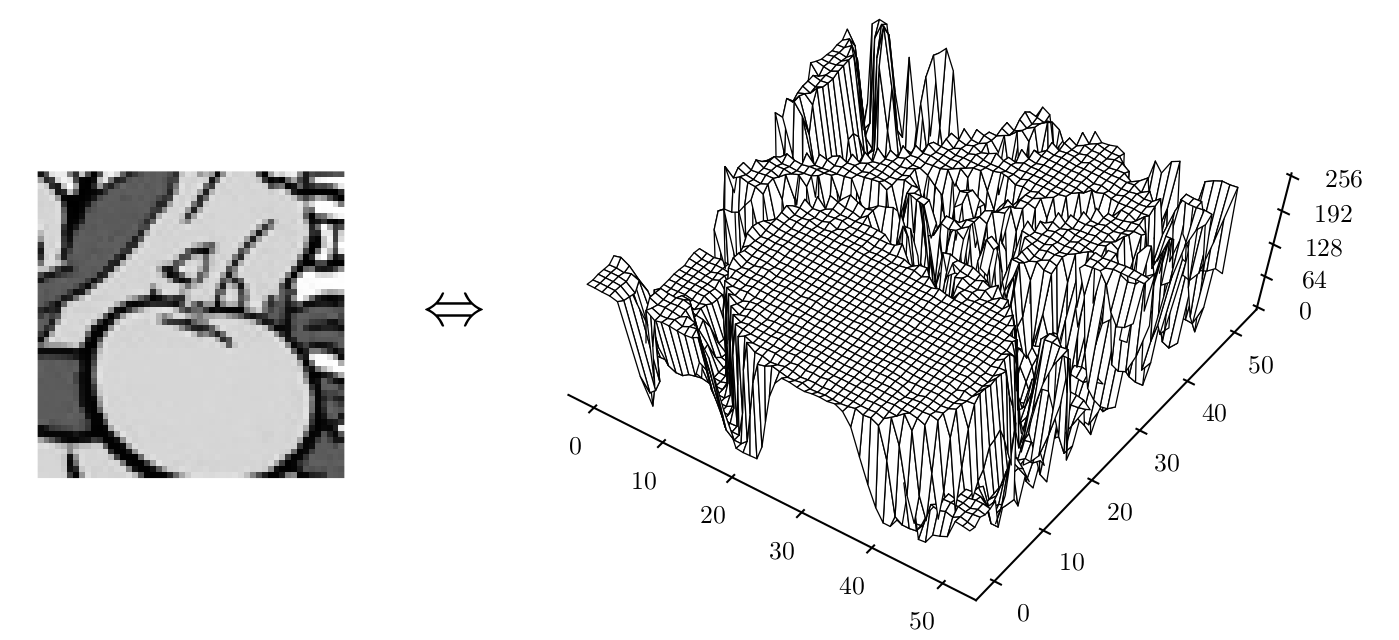
\includegraphics[width=0.9\linewidth]{images/ImageAsAFunctionExample}
	\caption{}
	\label{fig:imageasafunctionexample}
\end{figure}

\underline{Notation}: To signify that $f$ is continuous, write $f(x)$. To signify that $f$ is discrete (partial), write $f[x]$ (with $x\in \{\IR, \IR^2\}$).

\begin{Definition}[Derivatives]{def:Derivatives}
	Let $f$ be a continuous, uni-variate function $f:\IR\to\IR$ where $x\mapsto f(x)$ and $x_0\in \IR$.
	
	At $x_0$, the \textbf{derivative of} $f$ \textbf{from above} is
	\begin{equation} 
		f^\prime_+(x_0) = \lim\limits_{\epsilon\to 0}\frac{f(x_0 + \epsilon) - f(x_0)}{\epsilon} 
	\end{equation}
	At $x_0$, the \textbf{derivative of} $f$ \textbf{from below} is
	\begin{equation} 
		f^\prime_-(x_0) = \lim\limits_{\epsilon\to 0}\frac{f(x_0) - f(x_0-\epsilon)}{\epsilon} 
	\end{equation}
	
	$f$ is \textbf{differentiable} at $x_0$, if
	\begin{equation}
		f^\prime_+(x_0) = f^\prime_-(x_0) = f^\prime(x_0) = \frac{\partial}{\partial x} f(x_0)
	\end{equation}
	In this case, $f^\prime(x_0)$ indicates the \textit{rate of change} of $f$ at $x_0$. That is the \textit{slope of the tangent} of $f$ at $x_0$.
	
	$f$ is differentiable, if it is differentiable at any $x\in\IR$. 
	
	Note that the derivation is a \textbf{linear operator}~\footnote{An \textbf{operator} is a function that maps functions to functions.}:
	\begin{equation}
		\frac{\partial}{\partial x} \Big(af(x) + bg(x) \Big) = a\frac{\partial}{\partial x} f(x) + b\frac{\partial}{\partial x} g(x)
	\end{equation}
\end{Definition}

For the discrete case set for simplicity $x_{i+1} - x_i=1=\epsilon$. Then, the definitions are analogue:\begin{itemize}
	\item \textbf{Backward difference}:
	\begin{equation} 
		f^\prime_-[x] = \frac{f[x]-f[x-1]}{x-(x-1)} = f[x]-f[x-1]
	\end{equation}
	\item \textbf{Forward difference}:
	\begin{equation} 
		f^\prime_+[x] = \frac{f[x+1]-f[x]}{(x+1)-x} = f[x+1]-f[x]
	\end{equation}
	\item \textbf{Central difference}:
	\begin{equation} 
		f^\prime[x] = \frac{f^\prime_+[x]-f^\prime_-[x]}{2} = \frac{f[x+1]-f[x-1]}{2}
	\end{equation}
\end{itemize}

Note that if $f[x]$ has been sampled from $f(x)$, then the central difference of $f[x]$ provides a provably better approximation of the derivative of $f(x)$ than the backward- or forward differences.

Using an operator notation, we will also write the central difference as $f^\prime[x] = d_x f[x]$.

From this we can write the gradient for intensity images $f[x,y]$ as
\begin{equation}
	\nabla f[x,y] = \begin{bmatrix} d_x f[x,y]\\d_y f[x,y]\end{bmatrix}
	= \frac{1}{2} \begin{bmatrix} f[x+1,y]-f[x-1,y]\\f[x,y+1]-f[x,y-1]\end{bmatrix}
\end{equation}

\begin{figure}[H]
	\centering
	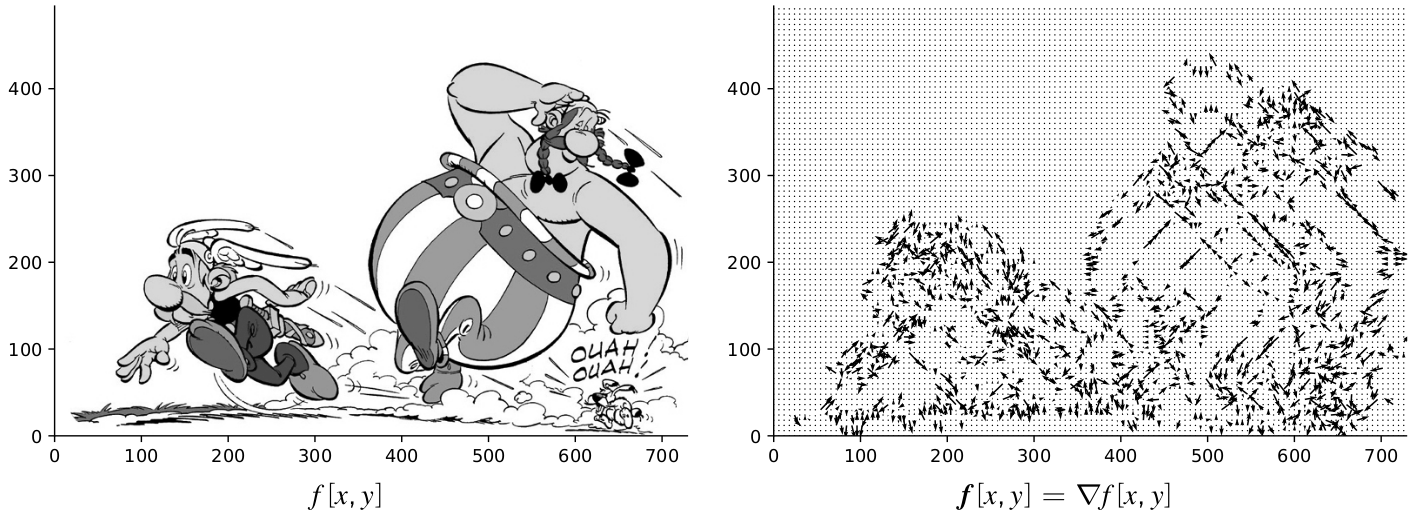
\includegraphics[width=0.9\linewidth]{images/GradientImageExample}
	\caption{Example intensity image and its gradient image.}
	\label{fig:gradientimageexample}
\end{figure}

%TODO: CONTINUE Slide 43

\chapter{Basics}


%%%%%%%%%%%%%%%%%%%%%%%%%%%%%%%%%%
%%%%% Lecture 02 - 18.10.2021 %%%%
%%%%%%%%%%%%%%%%%%%%%%%%%%%%%%%%%%

%%%%%%%%%%%%%%%%%%%%%%%%%%%%%%%%%%
%%%%% Lecture 03 - 25.10.2021 %%%%
%%%%%%%%%%%%%%%%%%%%%%%%%%%%%%%%%%

%%%%%%%%%%%%%%%%%%%%%%%%%%%%%%%%%%%%%%%%%%%%%%%%%%%%%%%%%%%%%%%%%%%%%%%%%%%%%%%%%%%%%%%%%%%%%%%%

%%%%%%%%%%%%%%%%%%%%%%%%%%%%%%%%%%%
%%%%% Lecture 0x of tt.mm.2021 %%%%
%%%%%%%%%%%%%%%%%%%%%%%%%%%%%%%%%%%


\newpage
%%%% ----------------------- %%%%
%%%% -------Exercises------- %%%%
%%%% ----------------------- %%%%

% !TeX spellcheck = en_GB 

\chapter{Exercises}
\section{Sheet 0 - Questions in the lecture slides}

\subsection{Q1 - lecture 02} 
Assume you have an RGB image of resolution $1024\times 768$ with $256$ intensity levels per color channel. How many bytes of memory does such an image require when loaded into a computer?
\paragraph{Solution:} 
To store $256=2^8$ intensity levels exactly eight bits (one byte) is required. Thus to store $1024\times 768 = 786,432$ pixels (intensity levels), \num[group-separator={,}]{786432} bytes are required.

\newpage
\section{Sheet 1}

\subsection{Assignment 1a - Bias of an estimator} 
\dots
\paragraph{Solution:} 


\newpage
%%%% ----------------------- %%%%
%%%% ------Bibliography----- %%%%
%%%% ----------------------- %%%%
\begin{thebibliography}{4}

\bibitem[1]{1}
\glqq EXAMPLE: Finite Elemente - Theorie, schnelle L�ser und Anwendungen in der Elastizit�tstheorie \grqq von Dietrich Braess, 5. Auflage, Springer, 2013

\end{thebibliography}

\end{document}
